\documentclass[tikz,border=2mm]{standalone}
\usepackage{pgfplots}
\pgfplotsset{compat=1.18}
\usetikzlibrary{arrows.meta}

\begin{document}
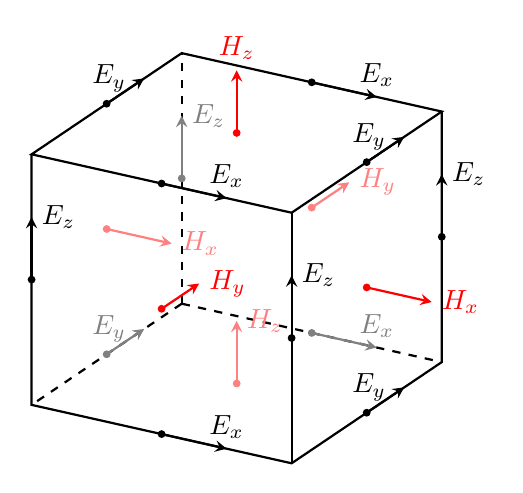
\begin{tikzpicture}
\begin{axis}[
    axis lines=none,          % Completely remove axis lines
    view={120}{25},
    width=12cm,
    height=12cm,
    xmin=-0.5, xmax=1.5,
    ymin=-0.5, ymax=1.5,
    zmin=-0.5, zmax=1.5,
    xtick=\empty,            % Remove x-axis numbers
    ytick=\empty,            % Remove y-axis numbers
    ztick=\empty,            % Remove z-axis numbers
    grid=none,               % Remove grid lines
    plot box ratio=1 1 1,
]

% Define cube vertices
\pgfmathsetmacro{\s}{1} % Cube size
\coordinate (O) at (0,0,0);
\coordinate (A) at (\s,0,0);
\coordinate (B) at (\s,\s,0);
\coordinate (C) at (0,\s,0);
\coordinate (D) at (0,0,\s);
\coordinate (E) at (\s,0,\s);
\coordinate (F) at (\s,\s,\s);
\coordinate (G) at (0,\s,\s);

% Draw cube edges
\draw[thick, dashed] (O) -- (A);
\draw[thick, dashed] (O) -- (C);
\draw[thick, dashed] (O) -- (D);
\draw[thick] (D) -- (E) -- (F) -- (G) -- cycle; % Top face
\draw[thick] (G) -- (C) -- (B) -- (A) -- (E);
\draw[thick] (B) -- (F);


%\node[anchor=south] at (axis cs:0,0,1.5) {$z$};
\node at (0,0,0.5)[circle,fill,black!50,inner sep=1pt]{};
\node at (1,0,0.5)[circle,fill,inner sep=1pt]{};
\node at (0,1,0.5)[circle,fill,inner sep=1pt]{};
\node at (1,1,0.5)[circle,fill,inner sep=1pt]{};

\node at (0,0.5,0)[circle,fill,black!50,inner sep=1pt]{};
\node at (1,0.5,0)[circle,fill,inner sep=1pt]{};
\node at (0.5,0,0)[circle,fill,black!50,inner sep=1pt]{};
\node at (0.5,1,0)[circle,fill,inner sep=1pt]{};

\node at (0,0.5,1)[circle,fill,inner sep=1pt]{};
\node at (1,0.5,1)[circle,fill,inner sep=1pt]{};
\node at (0.5,0,1)[circle,fill,inner sep=1pt]{};
\node at (0.5,1,1)[circle,fill,inner sep=1pt]{};



\node at (0,0.5,0.5)[circle,fill,red!50,inner sep=1pt]{};
\node at (1,0.5,0.5)[circle,fill,red,inner sep=1pt]{};
\node at (0.5,0,0.5)[circle,fill,red!50,inner sep=1pt]{};
\node at (0.5,1,0.5)[circle,fill,red,inner sep=1pt]{};

\node at (0.5,0.5,0.0)[circle,fill,red!50,inner sep=1pt]{};
\node at (0.5,0.5,1)[circle,fill,red,inner sep=1pt]{};


% arrows

\draw[-stealth,thick,red] (1,0.5,0.5) -- (0.75,0.5,0.5) node[right]{$H_y$};
\draw[-stealth,thick,red!50] (0.5,0,0.5) -- (0.5,0.25,0.5) node[right]{$H_x$};
\draw[-stealth,thick,red] (0.5,1,0.5) -- (0.5,1.25,0.5) node[right]{$H_x$};
\draw[-stealth,thick,red!50] (0,0.5,0.5) -- (-0.25,0.5,0.5) node[right]{$H_y$};


\draw[-stealth,thick,red] (0.5,0.5,1) -- (0.5,0.5,1.25) node[above]{$H_z$};
\draw[-stealth,thick,red!50] (0.5,0.5,0) -- (0.5,0.5,0.25) node[right]{$H_z$};




\draw[-stealth,thick,black!50] (0,0,0.5) -- (0,0,0.75) node[right]{$E_z$};
\draw[-stealth,thick,black] (1,0,0.5) -- (1,0,0.75) node[right]{$E_z$};
\draw[-stealth,thick,black] (0,1,0.5) -- (0,1,0.75) node[right]{$E_z$};
\draw[-stealth,thick,black] (1,1,0.5) -- (1,1,0.75) node[right]{$E_z$};



\draw[-stealth,thick,black!50] (0,0.5,0) -- (0,0.75,0) node[above]{$E_x$};
\draw[-stealth,thick,black] (1,0.5,0) -- (1,0.75,0) node[above]{$E_x$};
\draw[-stealth,thick,black!50] (0.5,0,0) -- (0.25,0,0) node[left=0.1cm]{$E_y$};
\draw[-stealth,thick,black] (0.5,1,0) -- (0.25,1,0) node[left=0.1cm]{$E_y$};

\draw[-stealth,thick,black] (0,0.5,1) -- (0,0.75,1) node[above]{$E_x$};
\draw[-stealth,thick,black] (1,0.5,1) -- (1,0.75,1) node[above]{$E_x$};
\draw[-stealth,thick,black] (0.5,0,1) -- (0.25,0,1) node[left=0.1cm]{$E_y$};
\draw[-stealth,thick,black] (0.5,1,1) -- (0.25,1,1) node[left=0.1cm]{$E_y$};

\end{axis}
\end{tikzpicture}
\end{document}